\chapter{Simulation par méthode de Cholesky}
\label{chapCholesky}
\section{Méthode de Cholesky}

\label{choleskySection1} En utilisant les notations du chapitre~\ref{introProb}, évoquons deux propriétés qui conduisent au premier algorithme de simulation
de la gaussienne $\mathcal{N}(0_{\mathbb{R}^{dm}},\Sigma)$.


\begin{property}
  Soit $r \in \mathbb{N}^{*}$ et $U_1, \cdots, U_r$ $r$ variables aléatoires réelles iid
suivant la loi gaussienne centrée réduite $\mathcal{N}(0,1)$. Alors:
\begin{center}
$U = (U_1, \cdots, U_r) \sim \mathcal{N}(0_{\mathbb{R}^r}, I_r)$
\end{center}
\end{property}

\begin{property}
Soit  $r \in \mathbb{N}^{*}$, $V: \Omega \rightarrow \mathbb{R}^r $ un vecteur aléatoire tel que $V \sim \mathcal{N}(0_{\mathbb{R}^r},~I_r)$, $A$ une matrice de $M_{r}(\mathbb{R})$, et $L$ une matrice triangulaire inférieure de $M_{r}(\mathbb{R})$ tel que 
\begin{equation}
A = LL^{T} \label{cholesky}
\end{equation}
 
\begin{center} Alors: $LV \sim \mathcal{N}(0_{\mathbb{R}^r},A)$ \end{center}
\end{property}

\begin{remark}
  La relation~\eqref{cholesky}  est la décomposition de Cholesky de $A$ par~$L$
\end{remark}


\noindent De ces propriétés, on obtient que si $\Sigma$ admet une décomposition de Cholesky et que l'on sait simuler des réalisations indépendantes
de la loi gaussienne univariée centrée réduite, alors on peut simuler $\mathcal{N}(0_{\mathbb{R}^{dm}},\Sigma)$.\\
~\\
Par une méthode du style Box-Muller, on sait simuler des réalisations indépendantes de la loi gaussienne univariée centrée réduite.
Puis comme $\Sigma$ est symétrique définie~positive, $\Sigma$ admet une décomposition de Cholesky $LL^{T}$.
Pour obtenir cette décomposition, on utilise la méthode de Cholesky qu'on peut appliquer à toute matrice réelle symétrique définie-positive.
(voir \textbf{Algorithme \ref{algo1}}). La décomposition de Cholesky est unique du moment que l'on impose à ce que les
coefficients diagonaux de $L$ soient des réels positives, ce que garantit la méthode de Cholesky. 

Finalement si on note $\Sigma = LL^{T}$, la décomposition de Cholesky de $\Sigma$, on déduit un algorithme de simulation
de $N$ réalisations indépendantes de $X_M$ (voir \textbf{Algorithme \ref{algo2}}).
~\\

\begin{algorithm}
\caption{\textsc{Méthode de Cholesky}}
\label{algo1}
\begin{algorithmic}
\REQUIRE {$A$ une matrice symétrique définie positive de taille $r$}
\BEGIN 
\STATE {Soit $L$ une matrice nulle de taille $r$}
\FOR {j:=1 \TO $r$}
\STATE {$L[j,j] = \sqrt{A[j,j]-\displaystyle\sum_{k=1}^{j-1} |L[j,k]|^{2}}$}
\FOR {i:=j+1 \TO $r$}
\STATE {$L[i,j] = \frac{A[i,j] - \displaystyle\sum_{k=1}^{j-1} L[j,k]L[i,k]}{L[j,j]}$}
\ENDFOR
\ENDFOR
\END
\ENSURE $L$ \\
\end{algorithmic}
\end{algorithm}

~\\
~\\



\begin{algorithm}
\caption{\textsc{Algorithme de simulation}}
\label{algo2}
\begin{algorithmic}
\REQUIRE $x$ liste de longueur $N$ (nombre de réalisations), $L \in M_{dm}(\mathbb{R})$ 
\BEGIN 
\FOR {i:=1 \TO $N$}  
\STATE {on produit $y = (y_1, \cdots, y_{dm})^{T} \in \mathbb{R}^{dm}$ selon  $\mathcal{N}(0_{\mathbb{R}^{dm}},I_{dm})$}
\STATE {$x[i] = Ly \in \mathbb{R}^{dm}$ (produit matriciel de $L$ et $y$)} 
\ENDFOR
\END
\ENSURE $x$ \\
\end{algorithmic}
\end{algorithm}
~\\
En observant l'algorithme~\ref{algo2}, on saisit que la complexité en temps d'une réalisation du vecteur gaussien $\mathcal{N}(0_{\mathbb{R}^{dm}},\Sigma)$ dépend de
si la matrice $L$ a été calculée ou non. Si c'est le cas, cette complexité se veut en $O((dm)^2)$ (produit matrice-vecteur). Si ce n'est pas
le cas, il faut aussi calculer la factorisation de Cholesky et la complexité en temps devient $O((dm)^3)$. La complexité
mémoire est en $O((dm)^2)$ (stockage de $\Sigma$).
\newpage
\section{Estimation de l'erreur}

\subsection{Quantification de l'erreur}
\label{quantifErreur}
Par la suite pour $r \in \mathbb{N}^{*}$, $\mathbb{R}^r$ pourra être vu comme l'ensemble des matrices colonnes à $r$ lignes.\\

Pour savoir si le vecteur aléatoire $X_M$ est bien simulé, il faut quantifier
une erreur de simulation. La loi forte des grands nombres stipule que si l'on considère $r$ un entier non nul, $(Y_N)_{N \in \mathbb{N}^{*}}$
une suite de vecteurs aléatoires dans $L^1_{\mathbb{R}^r}(\Omega,\mathbb{P})$ iid selon la loi d'un élément $Y \in L^1_{\mathbb{R}^r}(\Omega,\mathbb{P})$, alors:
\begin{center} $\frac{1}{N}\displaystyle\sum_{i = 1}^{N} Y_i  - \mathbb{E}(Y) \xrightarrow[N \to \infty]{p.s} 0$ \end{center}

\noindent Par conséquent si on considère $(Y_N)_{N \in \mathbb{N}^{*}}$ la suite de vecteurs aléatoires modélisant des réalisations indépendantes du vecteur aléatoire $X_M$, on a:
\begin{center} $\frac{1}{N}\displaystyle\sum_{i = 1}^{N} Y_iY_{i}^{T} \xrightarrow[N \to \infty]{p.s} \mathbb{E}(X_MX_{M}^{T}) = \Sigma $ \end{center}

\noindent Donc si on munit $M_{dm}(\mathbb{R})$ de la norme de Frobenius $ \|\cdot\|_F $, on obtient la reformulation suivante:
\begin{center} $\biggl \|\frac{1}{N}\displaystyle\sum_{i = 1}^{N} Y_iY_{i}^{T} - \Sigma \biggr\|_F \xrightarrow[N \to \infty]{p.s} 0 $ \end{center}

\noindent De ce résultat, on va pouvoir quantifier l'erreur de $N$ réalisations du vecteur $X_M \sim \mathcal{N}(0_{\mathbb{R}^{dm}},\Sigma) $, $y = (y_1, \cdots, y_N) \in~(\mathbb{R}^{dm})^N$, en introduisant la définition suivante.\\


\begin{definition}
Soit $N$ un entier naturel non nul et  $(z_1, \cdots, z_N) \in (\mathbb{R}^{dm})^N$ 
~\\
On définit alors l'erreur $L^2$ (relative à $X_M$) des $N$ réalisations $z=(z_1, \cdots, z_N)$ par la quantité:

\begin{equation*}
  \epsilon(\Sigma, z) = \frac{\biggl \|\frac{1}{N}\displaystyle\sum_{i = 1}^{N} z_iz_{i}^{T} - \Sigma \biggr \|_F}{\|\Sigma \|_F}
\end{equation*}
\end{definition}
~\\
\newpage
Ainsi, si on simule bien $X_M$, on a forcément par la loi forte des grands nombres, que plus le nombre de réalisations $N$ est grand, plus $\epsilon(\Sigma, y)$ doit tendre vers $0$.
L'erreur $L^2$ est donc un moyen de vérifier numériquement si notre façon de modéliser le vecteur $X_M$ est correct.\\

\subsection{Exemple sur la méthode de Cholesky}
Présentons un exemple concret où l'erreur $L^2$ a été calculée. On simule via Cholesky un processus
gaussien centré d'ordre 2 où $n = d = 1$ et ayant pour fonction de covariance $C(x,y) = e^{-|x-y|} \text{ pour } x,y \text{ dans } \mathbb{R} $.
On choisit ici $D=[-10,10]$ et comme maillage $M$, une subdivision régulière de $D$ en $1000$ intervalles ($M$~possède donc $1001$ n\oe uds).
Dans la figure~\ref{figCholeskyRea},  une réalisation de $X_M$ a été faite en les points du maillage. 

\begin{figure}[h]
\begin{center}
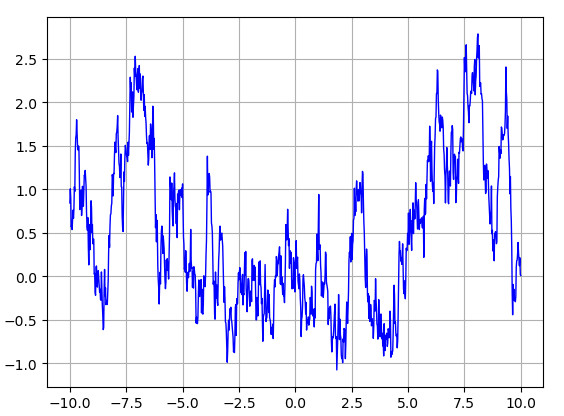
\includegraphics[scale=0.6]{images/ReaCholesky1D-1001nodes.jpg}
\caption{Réalisation du processus gaussien sur $[-10,10]$}
\label{figCholeskyRea}  
\end{center}
\end{figure}

\begin{table}[h]
\centering
\begin{tabular}{|c | c|}
\hline
Nb de réalisations & erreur $L^2$ \\
\hline
125 & 0.45627   \\
\hline
250  & 0.27285   \\
\hline
500  & 0.19814  \\
\hline
750  &  0.16260 \\
\hline
1000 &  0.15045 \\ 
\hline
\end{tabular}
\caption{Erreur $L^2$ en fonction du nombre de réalisations}
\end{table}


\begin{remark}
Le trait de la courbe de la figure~\ref{figCholeskyRea} se veut continue par interpolation linéaire en les points du maillage qui ont une valeur.
\end{remark}

\section{Erreur et convergence numérique}
\label{errConvCholesky}
La méthode de Cholesky nécessite un maillage $M$ et une fonction
de covariance $C$ pour déduire la matrice de covariance $\Sigma$. On se propose ici de décrire
les maillages et les fonctions de covariance utilisées pour les tests numériques.

\subsection{Dimension n=1}
\label{dimUnChol}
Pour les simulations, on a choisi $D = [-10,10]$. Pour $m \in \mathbb{N}^{*}, \; m > 1$,
les maillages considérés seront caractérisés à l'aide des n\oe uds du type
\begin{equation*} \biggl (t_i = -10 + \frac{20i}{m-1}\biggr)_{i \in \llbracket 0;m-1 \rrbracket}  \end{equation*}
et les éléments d'un maillage seront les intervalles de la forme $[t_i,t_{i+1}], \\i \in \llbracket 0;m-2 \rrbracket $.
On fera varier le nombre de n\oe uds $m$ entre $10$ et $10000$.\\
On n'associera à ces maillages qu'une seule fonction de covariance $C$:
\begin{equation*} C(x,y) = \exp(-|y-x|) \text{ pour } (x,y) \in \mathbb{R}^2 \end{equation*}

\begin{figure}[h]
\begin{center}
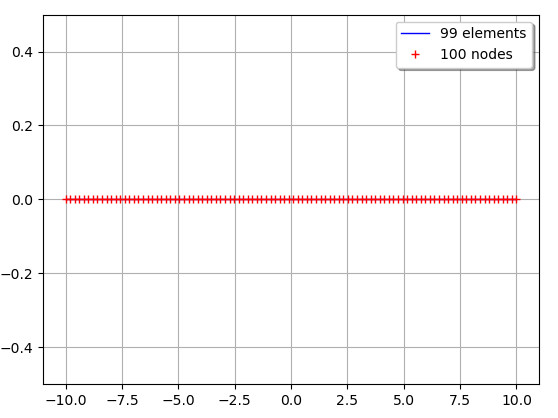
\includegraphics[scale=0.6]{images/CholeskyDim1-100.jpg}
\caption{Maillage à 100 n\oe uds en dimension 1}
\label{CholeskyMaillageDim1-100}  
\end{center}
\end{figure}


\subsection{Dimension n=2}
\label{choDim2}
En dimension 2, on a choisi $D = [-10,10]^2$. Pour $m \in \mathbb{N}^{*}, \; m > 1$,
les maillages considérés seront caractérisés par des n\oe uds du type
\begin{equation*} \biggl (t_{i,j} = (-10 + \frac{20i}{m-1}, -10 + \frac{20j}{m-1} )\biggr)_{(i,j) \in \llbracket 0;m-1 \rrbracket^2}  \end{equation*}
et par leurs éléments triangulaires dont les sommets sont décrits par des triplets
du type \begin{equation*}(t_{i,j}, t_{i+1,j}, t_{i,j+1}) \text{ ou } (t_{i+1,j}, t_{i+1,j+1}, t_{i,j+1}) , \; (i,j) \in \llbracket 0;m-2 \rrbracket^2 \end{equation*}
On fera varier le nombre de n\oe uds $m^2$ entre $10$ et $10000$.\\
On n'associera à ces maillages qu'une seule fonction de covariance $C$:
\begin{equation*} C(x,y) = \exp(-\|y-x\|_2) \text{ pour } (x,y) \in (\mathbb{R}^2)^2 \end{equation*}

\begin{figure}[h]
\begin{center}
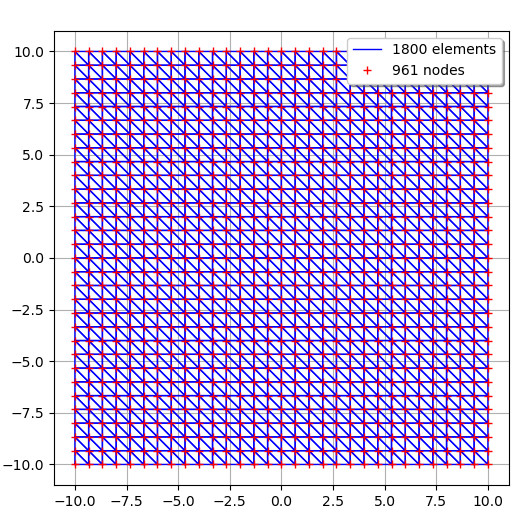
\includegraphics[scale=0.6]{images/CholeskyDim2-961.jpg}
\caption{Maillage à 961 n\oe uds en dimension 2}
\label{CholeskyMaillageDim2-961}  
\end{center}
\end{figure}

\subsection{Dimension n=3}
\label{choDim3}
En dimension 3, on a choisi $D = [-10,10]^3$. Pour $m \in \mathbb{N}^{*}, \; m > 1$,
les maillages considérés seront caractérisés par des n\oe uds du type
\begin{equation*} \biggl (t_{i,j,k} = (-10 + \frac{20i}{m-1}, -10 + \frac{20j}{m-1}, -10 + \frac{20k}{m-1} )\biggr)_{(i,j,k) \in \llbracket 0;m-1 \rrbracket^3}  \end{equation*}
et par leurs éléments tétraédriques dont les sommets sont décrits pour \\$(i,j,k) \in \llbracket 0;m-2 \rrbracket^3$ par des quadruplets ayant une de ces 6 formes:
\begin{equation*}(t_{i,j,k},\; t_{i+1,j,k},\; t_{i+1,j,k+1},\; t_{i+1,j+1,k+1}) , \end{equation*}
\begin{equation*}(t_{i,j,k},\; t_{i+1,j+1,k}, \;t_{i+1,j,k}, \;t_{i+1,j+1,k+1}) , \end{equation*}
\begin{equation*}(t_{i,j,k},\; t_{i+1,j,k+1},\; t_{i,j,k+1},\; t_{i+1,j+1,k+1}) , \end{equation*}
\begin{equation*}(t_{i,j,k},\; t_{i,j,k+1},\; t_{i,j+1,k+1}, \;t_{i+1,j+1,k+1}) , \end{equation*}
\begin{equation*}(t_{i,j,k},\; t_{i,j+1,k+1},\; t_{i,j+1,k},\; t_{i+1,j+1,k+1}) , \end{equation*}
\begin{equation*}(t_{i,j,k},\; t_{i,j+1,k},\; t_{i+1,j+1,k},\; t_{i+1,j+1,k+1}) \end{equation*}
On fera varier le nombre de n\oe uds $m^3$ entre $10$ et $10000$.\\
On n'associera à ces maillages qu'une seule fonction de covariance $C$:
\begin{equation*} C(x,y) = \exp(-\|y-x\|_2) \text{ pour } (x,y) \in (\mathbb{R}^3)^2 \end{equation*}
\phantom{oyez}

\begin{figure}[h]
\begin{center}
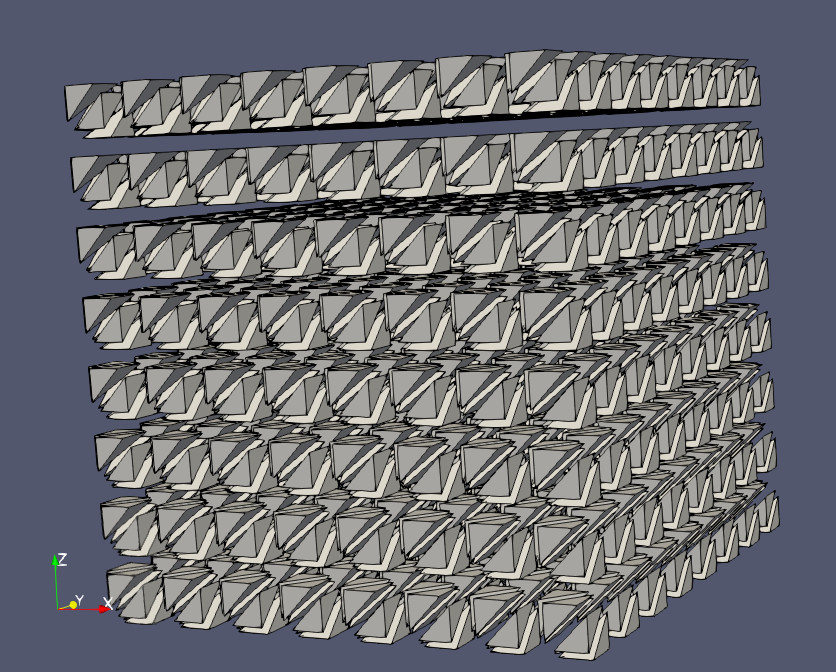
\includegraphics[scale=0.2]{images/CholeskyMaillageDim3-729.jpg}
\caption{Maillage à 729 n\oe uds en dimension 3}
\label{CholeskyMaillageDim3-729}  
\end{center}
\end{figure}


\subsection{Benchmarks}

\normalsize{
\begin{table}[htbp]
\footnotesize{
\begin{tabular}{|c |c |c |}
\hline
Dimension & Nb de n\oe uds & Temps moyen d'une réalisation (en secondes) \\
\hline
1 & 10 & 0.00020s    \\
\hline
1 & 100 & 0.00054s  \\
\hline
1 & 1000 & 0.16301s   \\
\hline
1 & 10000 & 183.51s    \\
\hline
\hline
2 & 9 & 0.00075s    \\
\hline
2 & 100 & 0.00084s    \\
\hline
2 & 961 & 0.19619s  \\
\hline
2 & 10000 & 164.28s   \\
\hline
\hline
3 & 8 & 0.00044s    \\
\hline
3 & 64 & 0.00060s    \\
\hline
3 & 729 & 0.05580s    \\
\hline
3 & 9261 & 116.86s  \\
\hline
\end{tabular}
}
%\caption{}
\end{table}
\newpage
\small{
\begin{remark}
Le nombre moyen de réalisations est estimé sur une durée de 5 secondes maximum.
Une durée supérieure à 5 secondes pointe le fait qu'une
seule réalisation a pu être effectuée et qu'elle a duré plus de 5 secondes.
Certes pour un grand maillage, la durée non négligeable de la factorisation de
Cholesky de $\Sigma$ augmente le temps de la première réalisation, mais bien souvent
les capacités limitées de la mémoire vive nécessitent de la
mémoire supplémentaire et l'accès à cette mémoire ralentit l'exécution
du code. Ceci explique notamment les temps moyens supérieures à 100 secondes. On note aussi
que pour un maillage donnée, l'erreur $L^2$ tend vers $0$ comme l'inverse de
la racine carrée du nombre de réalisations.\\
~\\
\end{remark}
}
\normalsize{}

\begin{table}[htbp]
\centering
\footnotesize{
\begin{tabular}{|c |c |c |c |c |} 
\hline
Dimension & Nb de n\oe uds & Nb de réalisations & erreur $L^2$ \\
\hline
1 & 10 & 250 & 0.14875   \\
\hline
1 & 10 & 500 & 0.12409    \\
\hline
1 & 10 & 750 &  0.09597   \\
\hline
1 & 10 & 1000 & 0.07025   \\
\hline
\hline
1 & 100 & 250 &  0.26887   \\
\hline
1 & 100 & 500 & 0.19460  \\
\hline
1 & 100 & 750 & 0.14790    \\
\hline
1 & 100 & 1000 & 0.13010    \\
\hline
\hline
1 & 1000 & 250 & 0.29682    \\
\hline
1 & 1000 & 500 & 0.18924    \\
\hline
1 & 1000 & 750 &  0.17071  \\
\hline
1 & 1000 & 1000 & 0.14616    \\
\hline
\hline
2 & 9 & 250 & 0.20574   \\
\hline
2 & 9 & 500 &  0.12867  \\
\hline
2 & 9 & 750 & 0.09212   \\
\hline
2 & 9 & 1000 & 0.09902  \\
\hline
\hline
2 & 100 & 250 & 0.45563   \\
\hline
2 & 100 & 500 & 0.31861   \\
\hline
2 & 100 & 750 & 0.26100    \\
\hline
2 & 100 & 1000 & 0.22472  \\
\hline
\hline
2 & 961 & 250 & 0.91385   \\
\hline
2 & 961 & 500 & 0.65045     \\
\hline
2 & 961 & 750 & 0.53042   \\
\hline
2 & 961 & 1000 & 0.45776    \\
\hline
\hline
3 & 8 & 250 & 0.15579  \\
\hline
3 & 8 & 500 & 0.11870    \\
\hline
3 & 8 & 750 & 0.09126    \\
\hline
3 & 8 & 1000 & 0.08644    \\
\hline
\hline
3 & 64 & 250 & 0.37056   \\
\hline
3 & 64 & 500 & 0.25594   \\
\hline
3 & 64 & 750 & 0.21249    \\
\hline
3 & 64 & 1000 & 0.18017    \\
\hline
\hline
3 & 729 & 250 & 1.1991   \\
\hline
3 & 729 & 500 & 0.84544    \\
\hline
3 & 729 & 750 & 0.69187    \\
\hline
3 & 729 & 1000 & 0.59801   \\
\hline
\end{tabular}
}
\end{table}
\normalsize{}

%\begin{remark}
%On note aussi que pour un maillage donnée, l'erreur $L^2$ tend bien vers $0$ comme l'inverse de
%la racine carrée du nombre de réalisations.
%\end{remark}
